\subsection{Mess-Server}
\label{section_Mess-Server}

Als Mess-Server wird ein BeagleBone Black von Texas Instruments eingesetzt. Dabei handelt es sich um einen kostengünstigen Einplatinencomputer mit offener Hardware. Damit ist es möglich, das BeagleBone Black auf individuelle Anforderungen anzupassen und selbst herzustellen. Auch gibt es eine große Community, die ständig die Entwicklung vorantreibt.
Er arbeitet mit einem AM335x 1GHz ARM® Cortex-A8 Prozessor, verfügt über 512MB DDR3 RAM und 4GB 8-bit eMMC internen Flash Speicher. Als Spannungsversorgung dient ein 5V 2A Netzteil.


\begin{figure}[H]
\begin{center}
\includegraphics[width=0.8\textwidth]{img/general/BeagleBoneBlack.jpg}
\caption{BeagleBone Black}
\label{figure_Beagleboneblack}
\end{center}
\end{figure}

Trotz der Kompaktheit des BeagleBone Black, bietet er ein ausreichendes Maß an Performance. Auf ihm kommt ein Debian-GNU/Linux Betriebssystem zum Einsatz. Damit ist es möglich die umfangreichen Debian-Funktionen wie die Paketverwaltung zu nutzen. Es bietet auch den Vorteil, dass eine große Ähnlichkeit zu PC-Distributionen wie Ubuntu besteht und somit einfacher nutzbar ist(vgl. \cite{schroeder2009embedded}).\\
Außerdem sind Linux Mechanismen einfach nutzbar. So kann das \ac{UART} Interface beispielsweise wie eine normale Datei beschrieben und gelesen werden.

\subsubsection{Hardware}


\begin{figure}[H]
\begin{center}
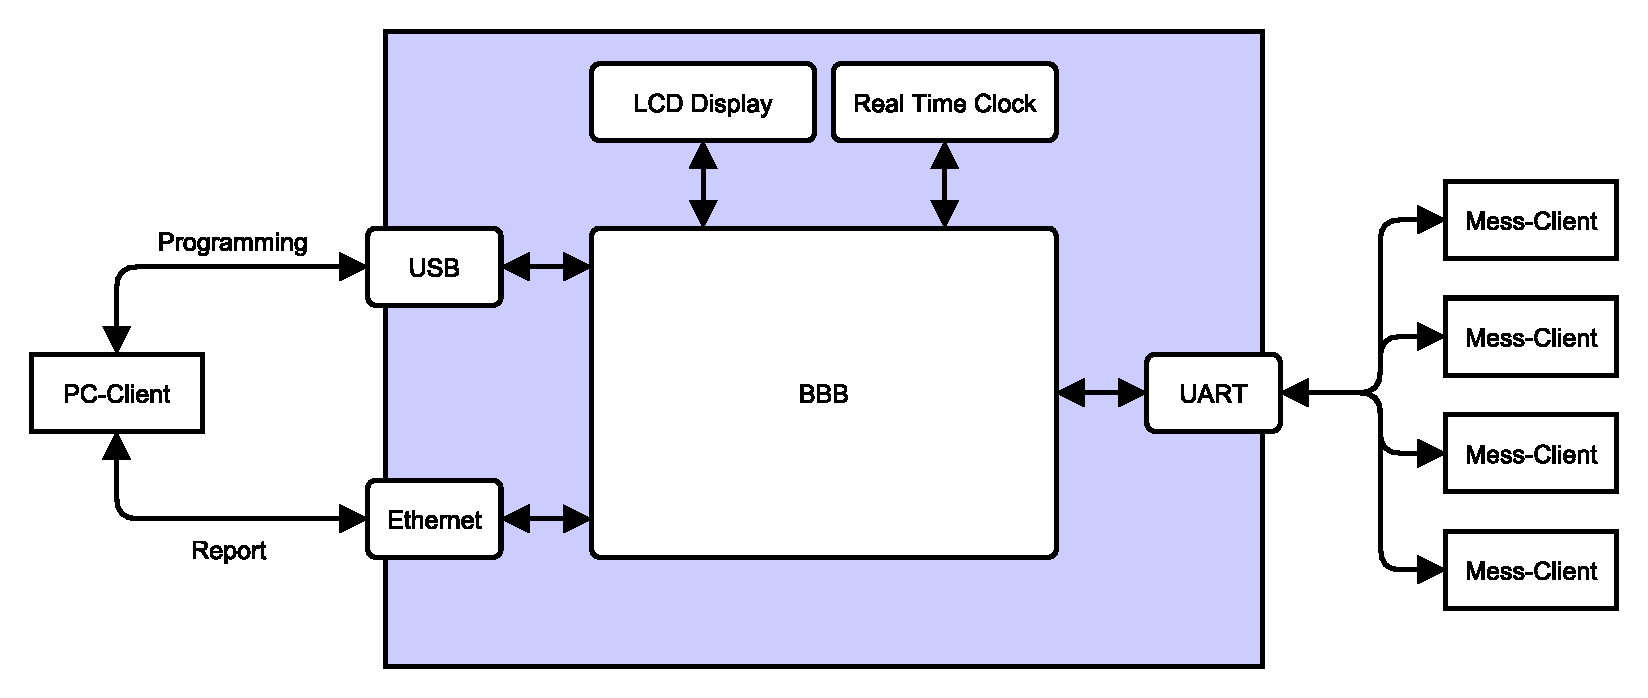
\includegraphics[width=\textwidth ]{img/general/UebersichtMaster.pdf}
\caption{Aufbau Mess-Server}
\label{figure_AufbauBleagleBone}
\end{center}
\end{figure}

Zur Kommunikation mit den Mess-Clients wird die \ac{UART} Schnittstelle des BeagleBone Black verwendet. Dafür wird ein RS232 Cape eingesetzt. Das Cape führt die seriellen Ports UART0, UART1, UART2 und UART4 auf einen 9-poligen seriellen Stecker. Es bietet die Möglichkeit zwischen den verschiedenen Ports mittels eines Jumper auf dem Cape zu wechseln.\\
Da das BeagleBone Black kein eigenes \ac{RTC} Modul besitzt, wird auch dieses durch ein Cape hinzugefügt. Es beinhaltet eine 3,3V Knopfbatterie um auch im Falle einer Stromunterbrechung die aktuelle Zeit nicht zu verlieren.\\
Um die Statusanzeige detailliert darstellen zu können, wird ein resistives LCD-Touchscreen Display eingesetzt. Es hat eine Größe von 4,3 Zoll bei einer Auflösung von 480x272 Pixeln. Dabei handelt es sich ebenso um ein Cape. Dadurch ist es möglich, das BeagleBone Black trotz den Erweiterungen kompakt zu halten. Denn die Capes sind untereinander Stapelbar.\\
Die USB Schnittstelle, welche zur Programmierung des BeagleBones verwendet wird, ist bereits vollständig einsatzbereit. Ebenso ist die Ethernet Schnittstelle, welche für den Fernzugriff auf das BeagleBone genutzt wird, bereits vollständig integriert.

\subsubsection{Software}

Die Programmierung der Software erfolgt in C++ unter Verwendung der Klassenbibliothek Qt (siehe Abschnitt \ref{section_Qt}).\\
Das Softwaredesign teilt sich in einen sequentiellen Teil für die Abfrage und Speicherung der Messwerte, sowie einen Event gesteuerten Teil für die \ac{GUI} und die externe Kommunikation für die Fernzugriffe.\\

Der Hauptzyklus der Software ruft kontinuierlich die Messdaten von den Mess-Clients ab.

$Aktuelle Zeit - Zeit letzter Messwert = Vergangene Zeit$


